
%(BEGIN_QUESTION)
% Copyright 2011, Tony R. Kuphaldt, released under the Creative Commons Attribution License (v 1.0)
% This means you may do almost anything with this work of mine, so long as you give me proper credit

An electric valve actuator using a permanent-magnet DC motor is configured to stop when a certain amount of seating force has been applied to the valve seat while moving in the ``shut'' direction.  This torque setting in the motor actuator is electronic in nature, but unfortunately there are no labels on the adjustment dial to show you how many foot-pounds or inch-pounds it is set for.  The actuator will stop automatically when closing, but you have no idea how much torque it is set to stop for.

To measure the actual closing-torque setting of this actuator, you connect a millivolt datalogger (trend recorder) in parallel with the shunt resistor that is built-in to the actuator, to allow you to measure motor current while it is running.  This shunt resistor has a value of 0.0025 ohms, and carries 100\% of the motor's current.  You know that any permanent magnet DC motor's torque is directly proportional to the amount of current it draws, and that this particular actuator is rated at 125 lb-ft of torque at a full-load motor current of 14.2 amps:

$$\includegraphics[width=15.5cm]{i01687x01.eps}$$

Based on the graphical results of this test (showing millivolts dropped across the motor shunt resistor over time), how many lb-ft of ``seating torque'' is the actuator set for?  Also, what does the ``hump'' in the middle of the graph indicate about the mechanical health of valve (please be specific!)?

\underbar{file i01687}
%(END_QUESTION)





%(BEGIN_ANSWER)

Half-credit for numerical answer, half credit for explanation of ``hump.''

\vskip 10pt

$\tau_{close}$ = 116.2 lb-ft

\vskip 10pt

The ``hump'' represents some form of opposition to stem movement, perhaps a region of friction in the packing or some interference between the moving plug and a something stationary.  A mechanical problem (binding?) in the actuator itself may also account for this temporary increase in motor current (torque).

%(END_ANSWER)





%(BEGIN_NOTES)

{\bf This question is intended for exams only and not worksheets!}.

%(END_NOTES)


